\documentclass[12 pt]{beamer}
\usepackage[utf8]{inputenc}

\usepackage[]{amssymb}

\usepackage{multimedia}
\usepackage{media9}

\title{Modelos matemáticos de la disonancia}
\author{\normalsize{Manuel Gijón Agudo}}
%\date{10 July 2017}
\date{}

\mode<presentation>{\usetheme{Madrid}}


\begin{document}

% TÍTULO
%\frame{\titlepage}   


\begin{frame}[plain]
    \begin{center}

        Universidad Politécnica de Cataluña
        
        Facultad de Matemáticas y Estadística
        
        Grado en Matemáticas
        
        \scriptsize{Trabajo de Final de Grado}
        
        \maketitle    
        Director: Xavier Gràcia Sabaté
    
        Departamento de Matemáticas\\*
        
        \small{10 Julio 2017}
    \end{center}
    
    
\end{frame}

% DEFINICIONES DE COLORES
\setbeamercolor{amarilloNota}{bg=yellow!50!white}
\setbeamercolor{azulNota}{bg=blue!15!white}
\setbeamercolor{naranjaNota}{bg=orange!15!white}


% DIAPOSITIVA 1 
\begin{frame}{1}

    \frametitle{Índice}
     
    \tableofcontents  % esto generará automáticamente el índice a partir de las section, subsection y subsubsection
\end{frame}

\section{El sonido y su percepción}

% DIAPOSITIVA 3
\begin{frame}{3}
    \frametitle{El sonido y su percepción}
  
    El estudio del sonido debe hacerse desde dos puntos de vista: el \emph{físico}, es un fenómeno medible y perfectamente cuantificable y el \emph{perceptivo}, las sensaciones que este produce en la persona que lo escucha y que conforman una experiencia subjetiva.
    
    \vspace{1cm}
    En los elementos que utilizamos para estudiar el sonido también estarán presentes estos dos enfoques.   
    
\end{frame}

\begin{frame}
    \frametitle{El sonido y su percepción}
    \framesubtitle{Elementos en el estudio del sonido}
    
    \begin{alertblock}{Elementos físicos}
        \begin{itemize}
            \item Intensidad
            \item Espectro
            \item Frecuencia
        \end{itemize}
    \end{alertblock}
    
    \pause
    
    \begin{exampleblock}{Elementos perceptivos}
        \begin{itemize}
            \item Sonoridad
            \item Timbre
            \item Altura
        \end{itemize}
    \end{exampleblock}
 %   \begin{beamercolorbox}[sep=5mm,center,rounded=true,shadow=true]{amarilloNota}
  %%         \item Intensidad
    %        \item Espectro
     %       \item Frecuencia
      %  \end{itemize}
    %\end{beamercolorbox}
%    \pause
 %   \begin{beamercolorbox}[sep=1mm,center,rounded=true,shadow=true]{azulNota}
  %      \begin{itemize}
   %         \item Sonoridad
    %        \item Timbre
     %       \item Altura
     %   \end{itemize}
    %\end{beamercolorbox}
    
    \end{frame}
% DIAPOSITIVA 4
%\begin{frame}{4}
%    \frametitle{El sonido y su percepción}
    
 %   \framesubtitle{Espectro y timbre}
    % TIMBRE
%    \begin{beamercolorbox}[sep=1mm,center,rounded=true,shadow=true]{amarilloNota}

%        ``El timbre es aquella cualidad de un sonido que nos hacer poder distinguirlo de otro de la misma altura.'' \cite{EH}
%    \end{beamercolorbox}
%    \pause
%    \begin{beamercolorbox}[sep=1mm,center,rounded=true,shadow=true]{azulNota}
        %A las frecuencias de las ondas sinusoidales que sumadas nos dan el sonido que estudiamos las llamaremos \emph{parciales} o \emph{armónicos}. El \emph{espectro} de un sonido será el conjunto formado por sus parciales y las amplitudes con las que estas se presentan.
%    \end{beamercolorbox}

%\end{frame}

% DIAPOSITIVA 5
%\begin{frame}{5}
 %   \frametitle{El sonido y su percepción}
%    \framesubtitle{Intensidad y sonoridad}


    %\begin{beamercolorbox}[sep=1mm,center,rounded=true,shadow=true]{amari%lloNota}
     %   La \emph{sonoridad} es la medida subjetiva de la intensidad con la que un sonido es percibido por el oído humano.
    %\end{beamercolorbox}
    %\pause
    %\begin{beamercolorbox}[sep=1mm,center,rounded=true,shadow=true]{azulNota}
        %La \emph{intensidad} de un sonido es una magnitud física. Se mide %en fons o fonios y su definición es:
    %    \begin{equation*}
        %    \boxed{
            %\textnormal{Intensidad} = \frac{\textnormal{Potencia %acústica}}{\textnormal{Área normal en la dirección de %propagación}}
            %}
  %      \end{equation*}
 %   \end{beamercolorbox}
   
%\end{frame}

% DIAPOSITIVA 6
%\begin{frame}{6}
 %   \frametitle{El sonido y su percepción}
  %  \framesubtitle{Frecuencia y altura}
    
  %  \begin{beamercolorbox}[sep=1mm,center,rounded=true,shadow=true]{amarilloNota}
   %     ``Aquel atributo en términos de la sensación sonora que hace posible dotar de un orden, de bajo a alto, diferentes sonidos''
        
    %    [American National Standards Institute]
%    \end{beamercolorbox}
%    \pause
%    \begin{beamercolorbox}[sep=1mm,center,rounded=true,shadow=true]{azulNota}
 %       La de \emph{frecuencia} de un sonido se corresponde con la frecuencia de la onda sinusoidal de su espectro que mayor amplitud tenga.
 %   \end{beamercolorbox}
        
%\end{frame}


\section{Consonancia y disonancia}

\subsection{El fenómeno de la disonancia}

% DIAPOSITIVA 7
\begin{frame}{7}
    \frametitle{Consonancia y disonancia}
    
    \framesubtitle{Disonancia}
    
    \begin{alertblock}{Disonancia}
    
        \begin{enumerate}
            \item Sonido desagradable.
            \item  Falta de la conformidad o proporción que naturalmente debe tener algo.
            \item Mús. Acorde no consonante.
        \end{enumerate}
        \begin{enumerate}
            \item loc. verb.  Parecer extraño y fuera de razón.
            [RAE]
        \end{enumerate}
        
    \end{alertblock}
    
\end{frame}


% DIAPOSITIVA 8
%\begin{frame}{8}
%    \frametitle{Consonancia y disonancia}
    
%    \framesubtitle{Diferentes teorías}
    
%    Estas son algunas de las teorías que explican el fenómeno y en las que no profundizaremos más adelante:
%    \begin{itemize}
%        \item Razones enteras: los intervalos cuyas razones están basadas en enteros simples y pequeños nos resultan más agradables.
%        \item Fusión: dos sonidos se percibirán más agradables cuanto más fácil puedan ser percibidos como uno solo.
%        \item Diferentes tonos: en ocasiones, dos sonidos sonando simultáneamente pueden dar lugar a la percepción de un tercer sonido. La posición de las parciales en este caso jugarán un papel fundamental en la consonancia o no del nuevo sonido.
%    \end{itemize}
    
%\end{frame}

\subsection{Hemlhotz}

% DIAPOSITIVA 9
\begin{frame}{9}
    \frametitle{Consonancia y disonancia}
    
    \framesubtitle{Interferencia entre ondas}
    
    La forma de interacción más simple entre dos sonidos es la \emph{interferencia}. Se produce cuando ambas tienen la misma frecuencia. Esta puede ser tanto constructiva como destructiva dependiendo de la fase de las ondas implicadas.
    
    \begin{figure}
        \centering
        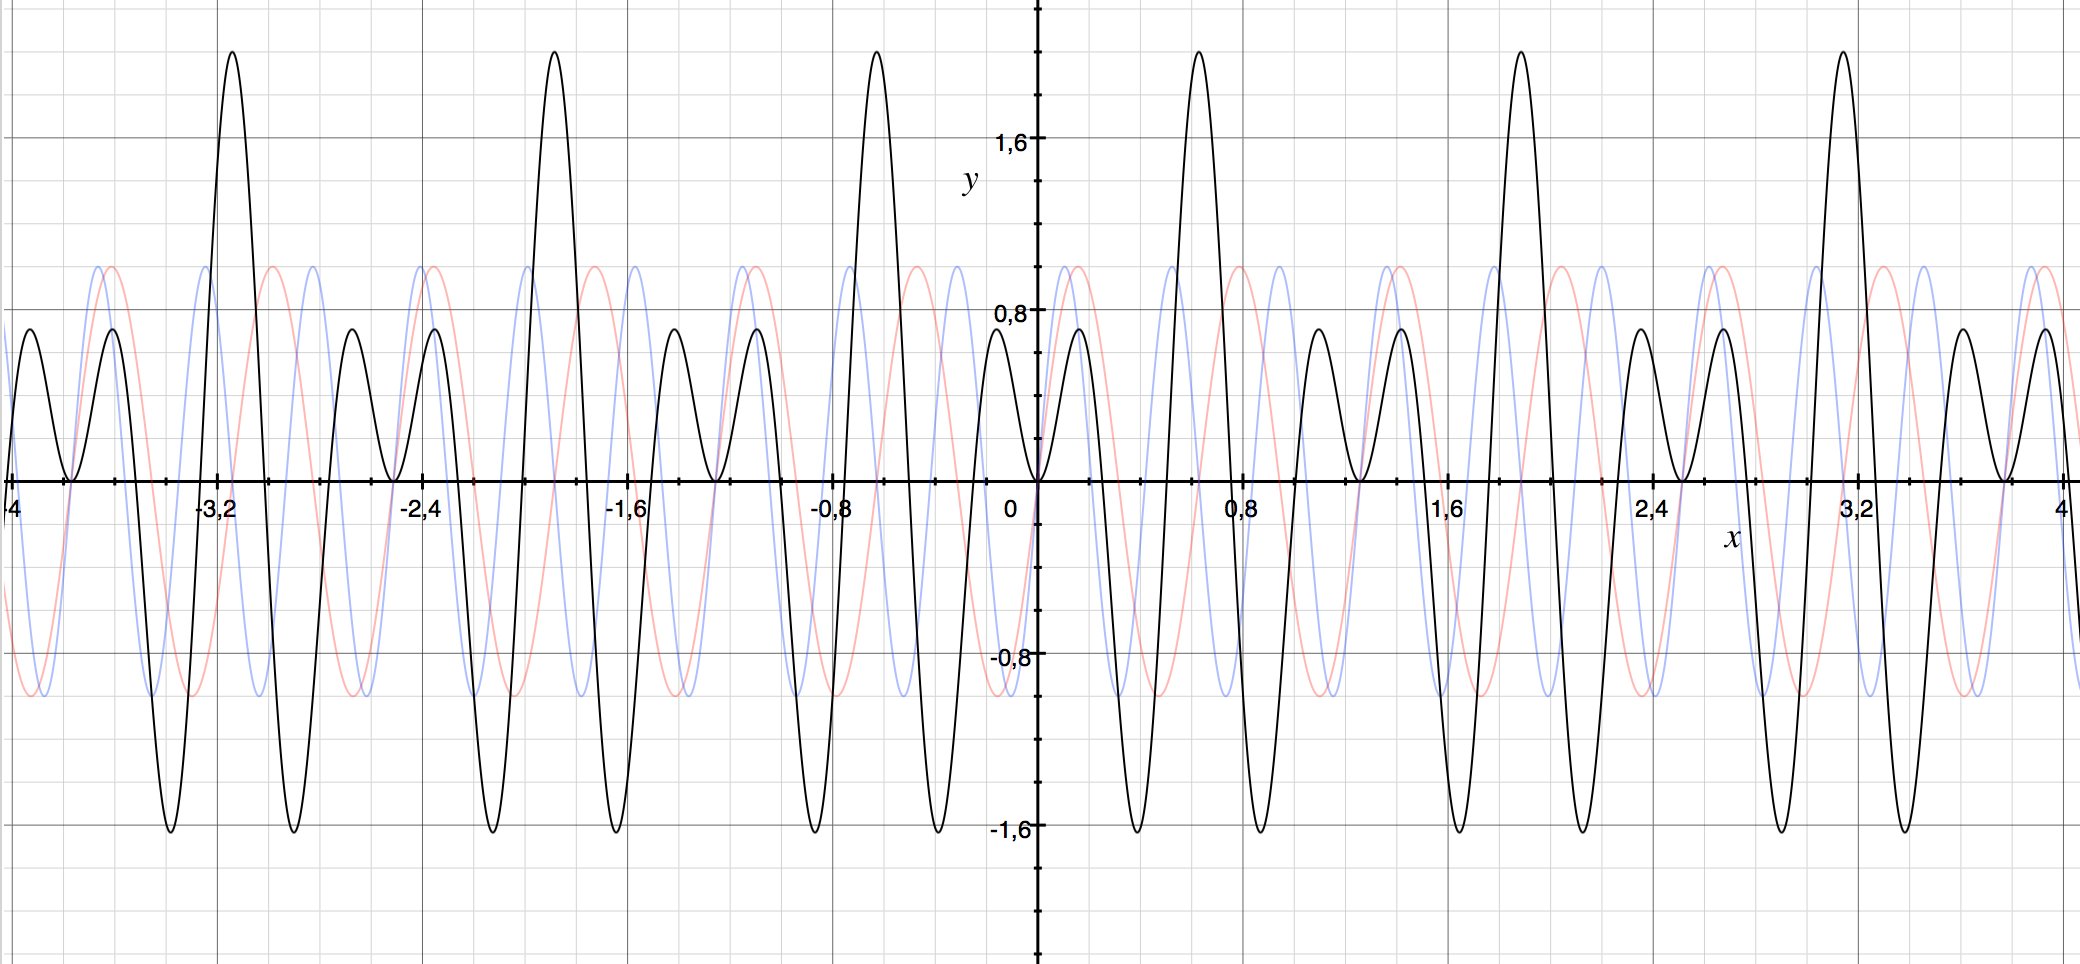
\includegraphics[scale = .2]{PiCuartosDiferenciaDeFase}
        \caption{Interacción entre ondas con ondas de misma frecuencia, $10$ Hz y una diferencia de fase de $\frac{\pi}{4}$}
    \end{figure}
        
\end{frame}

% DIAPOSITIVA 10
\begin{frame}{10}
    \frametitle{Consonancia y disonancia}
    
    \framesubtitle{Hemlhotz}
     
    La teoría de Hemlhotz es conocida como la teoría de los batidos. Esta dice que para dos ondas superponiéndose, en determinadas ocasiones puede producirse una cierta espereza que es interpretada como disonancia.
    
    Supongamos que tenemos dos ondas de frecuencias respectivas $\mu_1, \mu_2$, por ejemplo $\sin(2 \pi \mu_1 t)$ y $\sin(2 \pi \mu_2 t)$, su superposición vendría dada por:
    
    \begin{equation*}
        \boxed{
             \sin(2 \pi \mu_1 t) + \sin(2 \pi \mu_2 t) = 2 \sin\left( 2 \pi \frac{\mu_1 + \mu_2}{2} t \right) \cos \left( 2 \pi \frac{\mu_1 - \mu_2}{2} t \right)
        }
    \end{equation*}
\end{frame}

% DIAPOSITIVA 11
\begin{frame}{11}
    \frametitle{Consonancia y disonancia}
    
    \framesubtitle{Hemlhotz}
     
    \begin{itemize}
        \item Si la diferencia entre $\mu_1$ y $\mu_2$ es muy pequeña, se percibe como una onda de frecuencia $\mu = \frac{\mu_1 + \mu_2}{2}$ cuya amplitud varía con una frecuencia $\Delta \mu = |\mu_1 - \mu_2|$. En este caso se oirán los batidos.
        \item Si la diferencia es mayor, se producirá aspereza.
    \end{itemize}
    
\end{frame}

\subsection{Plomp y Levelt}

% DIAPOSITIVA 12
\begin{frame}{12}
    \frametitle{Consonancia y disonancia}
    
    \framesubtitle{R.Plomp y W.J.M.Level: el experimento}
    
    En 1965, con la idea de estudiar la consonancia de tonos complejos, Reinier Plomp y Willem J.M. Levelt llevaron a cabo el siguiente experimento \cite{PL}:
    
    \begin{itemize}
        \item Escogieron sujetos sin formación musical.
        \item Se emitieron tonos puros en frecuencias controladas.
        \item Se pedía a los sujetos que, haciendo uso de una escala determinada, valorasen el grado de disonancia (lo desagradable que les resultaban) los sonidos que estaban escuchando.
    \end{itemize}
    
    
\end{frame}

% DIAPOSITIVA 13
\begin{frame}{13}
    \frametitle{Consonancia y disonancia}
    
    \framesubtitle{R.Plomp y W.J.M.Level: el experimento}
    
    \begin{figure}
        \centering
        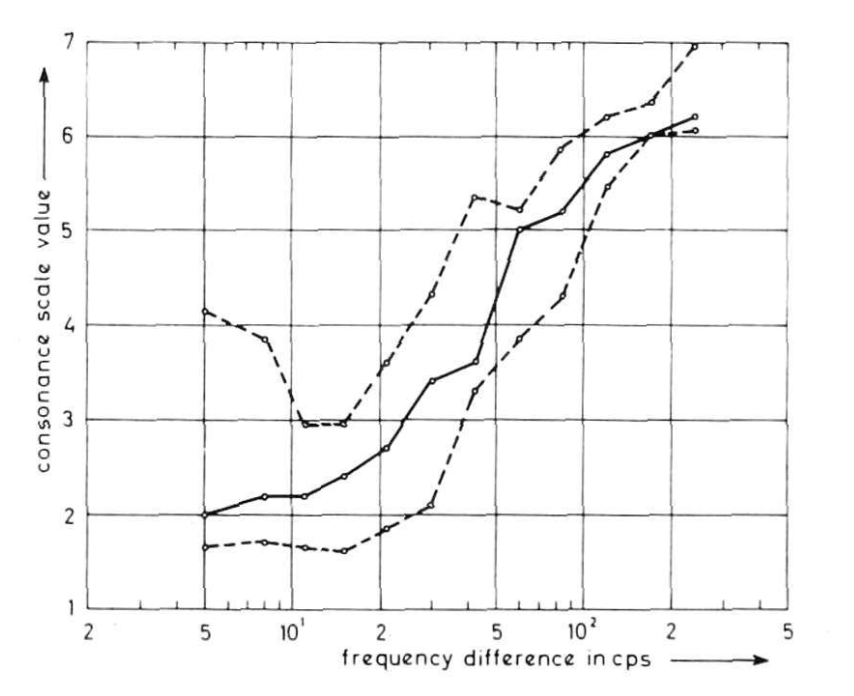
\includegraphics[scale = .5]{Datos1.png}
        \caption{Gráfica original del experimento de Plomp y Levelt \cite{PL}.}
    \end{figure}
    
\end{frame}

% DIAPOSITIVA 14
\begin{frame}{14}
    \frametitle{Consonancia y disonancia}
    
    \framesubtitle{R.Plomp y W.J.M.Level: resultados}
    
    \begin{block}{Resultados del experimento}
        \begin{itemize}
        \item El máximo de disonancia se produce a una distancia que no es fija, varía con la frecuencia siendo a una distancia aproximada de $\frac{1}{4}$ del ancho de banda crítica para esa frecuencia.
        \item A partir de ese punto, la consonancia aumenta, siendo el intervalo consonante a una distancia de ancho de banda crítica.
        %\item La gráfica muestra mínimos de disonancia locales en las razones de frecuencias simples $1:1, 1:2, 2:3, 3:5, 3:4, 5:6, 4:5$.
        %\item Al aumentar el número de parciales que conforman el espectro aparecen más mínimos de disonancia.
    \end{itemize}
    \end{block}
    
        
\end{frame}



\section{Estudio de las curvas de disonancia}

\subsection{El modelo propuesto por Sethares} 

% DIAPOSITIVA 15
\begin{frame}{15}
    \frametitle{Estudio de las curvas de disonancia}
    
    \framesubtitle{El modelo de Sethares}
    
    La siguiente definición es adecuada para el modelo que nos ocupa, más adelante la completaremos.
    
    \textbf{Definición 1:} dominaremos \emph{función de disonancia} a una funcion $d: \mathbb{R}^2 \rightarrow \mathbb{R}^{+}$ que se adapta a nuestros datos, devolviéndonos la disonancia entre dos frecuencias.
    
    En ocasiones, nos será más útil tener esta función como una función $d: \mathbb{R} \rightarrow \mathbb{R}$, para ello nos serviremos de una función que nos convierta dos frecuencias en un solo valor. Sethares utiliza la siguiente:
    
    \begin{equation*}
        x_{i,j} := \frac{|f_i - f_j|}{\min{ (f_i, f_j)} }
    \end{equation*}
    
\end{frame}

% DIAPOSITIVA 16
\begin{frame}{16}
 
    \frametitle{Estudio de las curvas de disonancia}
    
    \framesubtitle{El modelo de Sethares}
    
    La función de disonancia utilizada por el autor para parametrizar los resultados de  Plomp-Levelt tiene,si tomamos las amplitudes iguales y con valor $1$, la siguiente expresión:
    
    \begin{equation*}
        \boxed{
            d(x) := e^{-b_1 x} - e^{-b_2 x}
        }
    \end{equation*}
    
    con $b_1 = 3,5$ y $b_2 = 5,75$.
    
    \centering{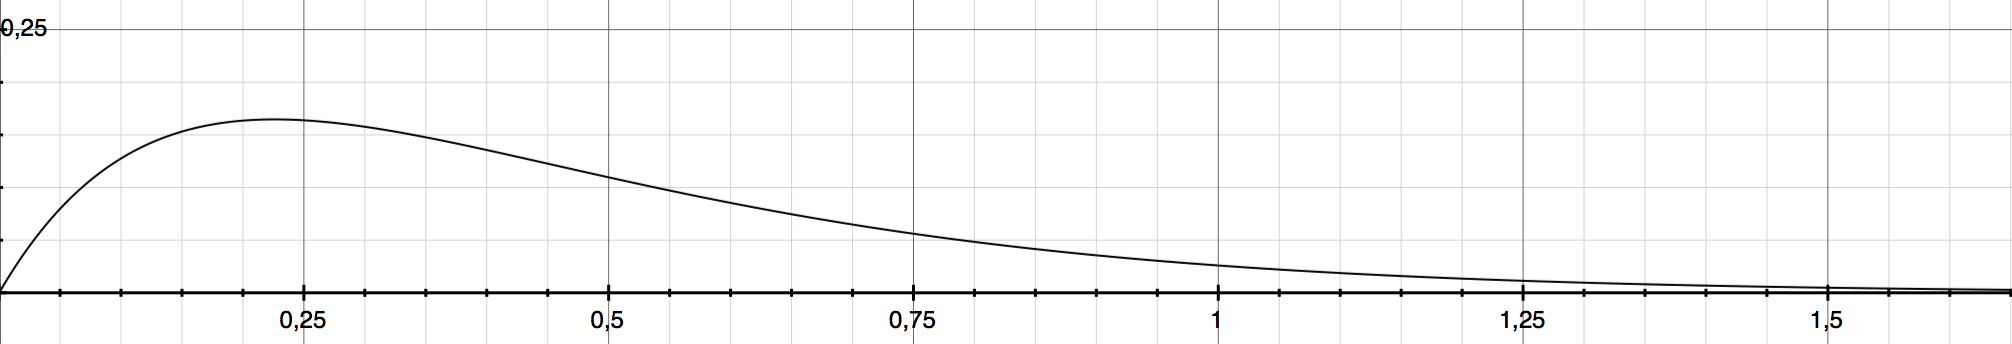
\includegraphics[scale = 0.3]{CurvaPlompLevelt}}
    
\end{frame}

% DIAPOSITIVA 17
\begin{frame}{17}
    \frametitle{Estudio de las curvas de disonancia}
    
    \framesubtitle{Algunas definiciones}
    
    \textbf{Definición 2:} Llamaremos \emph{timbre} o \emph{espectro} $\mathfrak{F}$ a una colección de $N$ frecuencias $f_1 < f_2 < ... < f_N$ con sus respectivas amplitudes. En nuestro caso todas serán iguales, simplificaremos la notación.
    \begin{equation*}
        \mathfrak{F} := \{ (f_i, l_i)\ : i = 1,2,..., N\} = \{ f_i : i = 1,2, ..., N\}  
    \end{equation*}
    
    \textbf{Definición 3:} Denominaremos \emph{espectro armónico} a aquel espectro cuyas parciales son múltiplos enteros de la frecuencia fundamental.
    
    \begin{equation*}
       \mathfrak{F}_{A} := \{ (f_i, l_i) : f_i = i\,f_{fundamental}\,, i =1, 2, ..., N   \}
    \end{equation*}
    
\end{frame}

% DIAPOSITIVA 18
\begin{frame}{18}
    \frametitle{Estudio de las curvas de disonancia}
    
    \framesubtitle{Algunas definiciones}
    
    
    \textbf{Definición 4:} Definimos la \emph{disonancia intrínseca del espectro $\mathfrak{F}$}  como:
    \begin{equation*}
        D_{\mathfrak{F}} := \frac{1}{2} \sum_{i}^{N} \sum_{j}^{N} d(f_i, f_j)
    \end{equation*}
    
    \textbf{Definición 5:} Denominaremos \emph{curva de disonancia generada por el espectro $\mathfrak{F}$} a la siguiente función:
    \begin{equation*}
        \boxed{
            D_{\mathfrak{F}} (\alpha) := D_{\mathfrak{F}} + D_{\mathfrak{\alpha F}} + \sum_{i}^{N} \sum_{j}^{N} d(f_i, \alpha f_j)
        }
    \end{equation*}
   siendo $\alpha \mathfrak{F} = \{ \alpha f_i : \forall f_i \in \mathfrak{F}\}$.
\end{frame}

% DIAPOSITIVA 19
\begin{frame}{19}
    \frametitle{Estudio de las curvas de disonancia}
    
    \framesubtitle{Hipótesis sobre el modelo}
        
    \begin{block}{Hipótesis}
        \begin{itemize}
            \item La suma total de la disonancia de un tono complejo es la suma de las disonancias parciales.
            \item Ambos espectros tendrán espectros en los que las parciales se distribuyen de la misma manera, es decir, un espectro será un múltiplo del otro.
            \item En estos espectros, para todas las parciales la amplitud será igual y la tomaremos con valor $1$.        
        \end{itemize}
    \end{block}
    
\end{frame}

% DIAPOSITIVA 20
\begin{frame}{20}
    \frametitle{Estudio de las curvas de disonancia}
    
    \framesubtitle{Ejemplos: espectros armónicos con 2 y 3 parciales}
    \begin{center}
        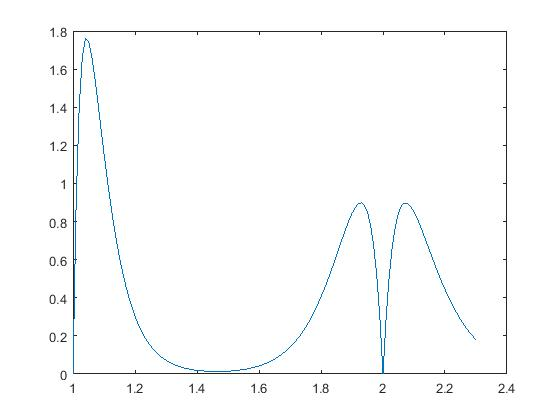
\includegraphics[scale = .30]{Espectro1_2}
        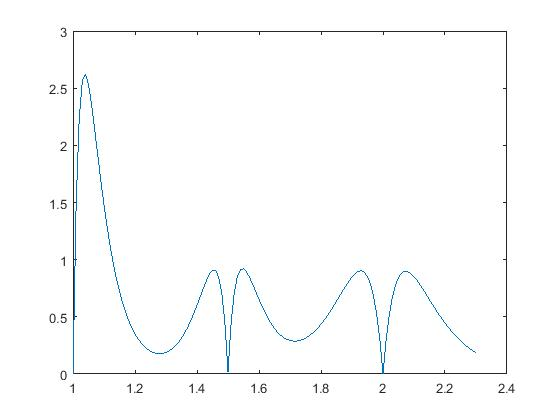
\includegraphics[scale = .30]{Espectro1_3}
    \end{center}
\end{frame}

% DIAPOSITIVA 21
\begin{frame}{21}
    \frametitle{Estudio de las curvas de disonancia}
    
    \framesubtitle{Ejemplos: espectros armónicos con 5 y 20 parciales}
    
    \begin{center}
        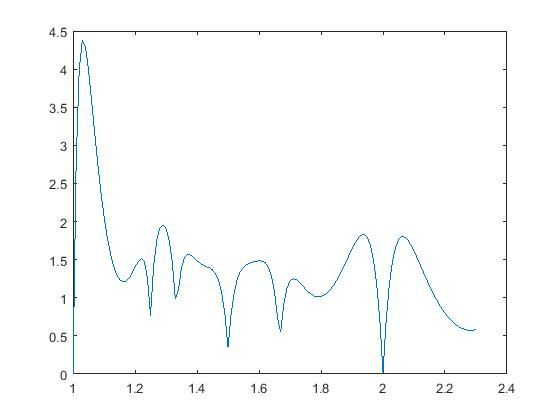
\includegraphics[scale = .3]{Espectro1_5}
        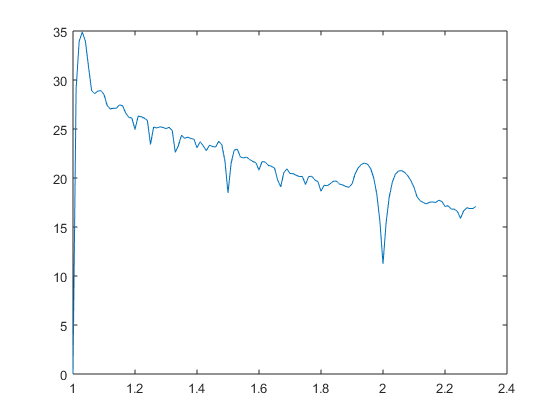
\includegraphics[scale = .4]{Espectro1-20}
    \end{center}
 %   \begin{figure}
 %      \centering
 %      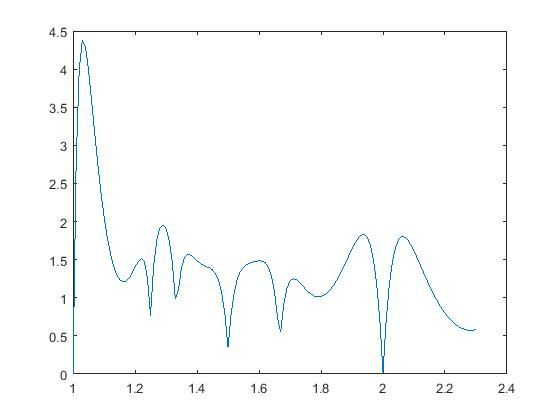
\includegraphics[scale = .5]{Espectro1_5}
 %      \caption{}
 %   \end{figure}
    
\end{frame}


\subsection{Una generalización de los resultados de Sethares}

\begin{frame}
    \frametitle{Estudio de las curvas de disonancia}
    \framesubtitle{Dos resultados sobre el modelo de Sethares}
    
    Los siguientes son resultados sobre el modelo utilizado por Sethares:
    \begin{equation*}
        \boxed{
            d(x) := e^{-b_1 x} - e^{-b_2 x}
        }
    \end{equation*}
    \begin{alertblock}{Resultado 1}
    \centering {$d^{(n)} (n x^{*}) = 0$, para todo $n \in \mathbb{N}$}, siendo $x^{*} \approx 0,22064$.
    \end{alertblock}
    
    \textbf{Idea de la demostración:} Observamos que $d \in \mathcal{C}^{\infty}$. Hallamos la expresión general de la derivada. Igualamos a cero y despejamos.
    
\end{frame}

\begin{frame}
    \frametitle{Estudio de las curvas de disonancia}
    \framesubtitle{Dos resultados sobre el modelo de Sethares}
    
    \begin{alertblock}{Resultado 2}
        \begin{enumerate}
            \item $d^{(n)}$ si $n$ es par alcanza su máximo en $(n+1)x^{*}$ y además $d^{(n)}((n+1)x^{*}) > 0$.
            \item $d^{(n)}$ si $n$ es impar alcanza su mínimo en $(n+1)x^{*}$ y además $d^{(n)}((n+1)x^{*}) < 0$.
        \end{enumerate}
    \end{alertblock}
    
    \textbf{Idea de la demostración:} Teniendo presente el resultado anterior lo único que resta demostrar es que la alternancia entre máximos y mínimos se sucede de la forma indicada.
    Nos fijamos en que $d'(x) > 0$ en $(0,x^{*})$ y $d'(x)<0$ a partir de ese punto. Observemos que se irá produciendo alternancia entre las regiones positivas y negativas.
    
\end{frame}

% DIAPOSITIVA 22
\begin{frame}{22}
    \frametitle{Estudio de las curvas de disonancia}
    
    \framesubtitle{Versión general de las curvas de disonancia}
    
    La siguiente es una definición más general de la función de disonancia.
    
    \begin{alertblock}{}
    Una \emph{función de disonancia} $d: \mathbb{R} \rightarrow \mathbb{R}$ es una función que cumple:
    
    \begin{enumerate}    
        \item $d \in \mathcal{C}^{1} (0, + \infty)$.
        \item $d(x) \geq q x $ con $q \geq 0$ en un entorno de $0$.
        \item $d'(x) \geq  -M$, $\forall x \in (0, + \infty)$ con $M > 0$.
        \item $d$ creciente en $ [0, x^{*})$, es decir, $d'(x) > 0$ para $x \in  [0, x^{*})$.
        \item $d$ decreciente en $(x^{*}, + \infty )$, es decir, $d'(x) < 0$ para $x \in (x^{*}, + \infty )$.
        \item La función tiene un máximo absoluto en $x^*$.
        \item $\lim_{x \rightarrow 0} d(x) = 0$ y también $\lim_{x \rightarrow +\infty} d(x) = 0$ 
    \end{enumerate}
    
    \end{alertblock}
    
    Notemos que en el modelo de Sethares $q\approx2,25$ y $M\approx2,33 \cdot10^{-3}$.
\end{frame}

% DIAPOSITIVA 23
\begin{frame}{23}
    \frametitle{Estudio de las curvas de disonancia}
    
    \framesubtitle{Resultado sobre el unísono como mínimo}
    
    A diferencia de Sethares, la función que utilizaremos para obtener un valor que introducir en la función de disonancia a partir de dos parciales será:
    
    \begin{equation*}
        x_{i,j} := \frac{|f_i - f_j|}{\mathcal{C} \min{(f_i, f_j)}}
    \end{equation*}
    
    Que, ajustando el valor de la constante $\mathcal{C}$ a las frecuencias implicadas, nos dirá la distancia medida en anchos de banda críticos entre las parciales. Una buena aproximación es tomar $\mathcal{C} = 0,17$.
    
    En nuestro caso, dejaremos fijas las parciales y para cada pareja nuestra variable será la razón $\alpha$, nos quedará por tanto:
    
    \begin{equation*}
        \boxed{
            x_{i,j}(\alpha) := \frac{|f_i - \alpha f_j|}{\mathcal{C}  \min{(f_i, \alpha f_j)}}
        }
    \end{equation*}
    
\end{frame}

% DIAPOSITIVA 24
\begin{frame}{24}
    \frametitle{Estudio de las curvas de disonancia}
    
    \framesubtitle{Resultado sobre el unísono como mínimo}
    
    \begin{alertblock}{Teorema: el unísono como mínimo de la disonancia}
    Sea $d$ una función de disonancia. Sea $\mathfrak{F} = \{ f_i : i = 1, 2,... , N\}$ un timbre con $N$ parciales, todas ellas de amplitud $1$. Entonces $\alpha = 1$ es un mínimo de la curva de disonancia.
    \end{alertblock}
    
    \textbf{Idea de la demostración:} No podemos derivar, luego para comprobar que tenemos un mínimo deberemos comprobar que, en torno al punto que nos interesa el cambio en la función es positivo sea cual sea el espectro. Las condiciones ($2$) y ($3$) de la definición de función de disonancia nos permitirán controlar estas variaciones, teniendo en cuenta que siempre las disonancias intrínsecas serán constantes.
\end{frame}

\section{Conclusiones}
% DIAPOSITIVA 25
\begin{frame}{25}
    \frametitle{Conclusiones}
    
    \begin{itemize}
        \item Hemos estudiado un modelo más general que para la curva de disonancia que el propuesto por Sethares basándose en los trabajos de Plomp y Levelt.
        \item Para este, hemos probado un teorema que garantiza que para un espectro sin límite en el número de parciales, el unísono será un mínimo de la curva de disonancia.
        \item Además, hemos establecido dos resultados que nos caracterizan más aún el modelo de Sethares.
    \end{itemize}
    
    Para el futuro, quedan como posibles trabajos:
    \begin{itemize}
        \item Extender los resultados a espectros con amplitudes variables.
        \item Generalizar el modelo a dimensiones mayores, las denominadas superficies de disonancia.
    \end{itemize}
\end{frame}

% DIAPOSITIVA 26
\begin{frame}{26}
    \frametitle{Bibliografía}
    
    
    \begin{thebibliography}{ABC9999}

    \bibitem[Ben]{Bens}
    D.\,J. Benson,
    \textit{Music: A Mathematical Offering}, 
        Cambridge University Press, 2008.
        %http://www.maths.abdn.ac.uk/∼bensondj/
	    
    \bibitem[PL]{PL}
    R. Plomp y W.\,M. Levelt
    ``Total Consonance and Critical Bandwidth''
        \textit{Institute for Perception TVO-TNO}, Soeslerberg, Nethrlands (1965)

    \bibitem[Set]{Set}
    W. Sethares,
        \textit{Tuning, Timbre, Spectrum, Scale}, 2nd ed,
        Springer, 2005.

    \bibitem[Set']{AT}
    W.\,A. Sethares
    ``Adaptative tunings for musical scales'',
        \textit{J. Acoustic Society of America} \textbf{96} (July, 1994)


\end{thebibliography}
        
\end{frame}

\end{document}
